% Options for packages loaded elsewhere
\PassOptionsToPackage{unicode}{hyperref}
\PassOptionsToPackage{hyphens}{url}
%
\documentclass[
  ignorenonframetext,
  aspectratio=169,
]{beamer}
\usepackage{pgfpages}
\setbeamertemplate{caption}[numbered]
\setbeamertemplate{caption label separator}{: }
\setbeamercolor{caption name}{fg=normal text.fg}
\beamertemplatenavigationsymbolsempty
% Prevent slide breaks in the middle of a paragraph
\widowpenalties 1 10000
\raggedbottom
\setbeamertemplate{part page}{
  \centering
  \begin{beamercolorbox}[sep=16pt,center]{part title}
    \usebeamerfont{part title}\insertpart\par
  \end{beamercolorbox}
}
\setbeamertemplate{section page}{
  \centering
  \begin{beamercolorbox}[sep=12pt,center]{part title}
    \usebeamerfont{section title}\insertsection\par
  \end{beamercolorbox}
}
\setbeamertemplate{subsection page}{
  \centering
  \begin{beamercolorbox}[sep=8pt,center]{part title}
    \usebeamerfont{subsection title}\insertsubsection\par
  \end{beamercolorbox}
}
\AtBeginPart{
  \frame{\partpage}
}
\AtBeginSection{
  \ifbibliography
  \else
    \frame{\sectionpage}
  \fi
}
\AtBeginSubsection{
  \frame{\subsectionpage}
}

\usepackage{amsmath,amssymb}
\usepackage{iftex}
\ifPDFTeX
  \usepackage[T1]{fontenc}
  \usepackage[utf8]{inputenc}
  \usepackage{textcomp} % provide euro and other symbols
\else % if luatex or xetex
  \usepackage{unicode-math}
  \defaultfontfeatures{Scale=MatchLowercase}
  \defaultfontfeatures[\rmfamily]{Ligatures=TeX,Scale=1}
\fi
\usepackage{lmodern}
\ifPDFTeX\else  
    % xetex/luatex font selection
\fi
% Use upquote if available, for straight quotes in verbatim environments
\IfFileExists{upquote.sty}{\usepackage{upquote}}{}
\IfFileExists{microtype.sty}{% use microtype if available
  \usepackage[]{microtype}
  \UseMicrotypeSet[protrusion]{basicmath} % disable protrusion for tt fonts
}{}
\makeatletter
\@ifundefined{KOMAClassName}{% if non-KOMA class
  \IfFileExists{parskip.sty}{%
    \usepackage{parskip}
  }{% else
    \setlength{\parindent}{0pt}
    \setlength{\parskip}{6pt plus 2pt minus 1pt}}
}{% if KOMA class
  \KOMAoptions{parskip=half}}
\makeatother
\usepackage{xcolor}
\newif\ifbibliography
\setlength{\emergencystretch}{3em} % prevent overfull lines
\setcounter{secnumdepth}{-\maxdimen} % remove section numbering


\providecommand{\tightlist}{%
  \setlength{\itemsep}{0pt}\setlength{\parskip}{0pt}}\usepackage{longtable,booktabs,array}
\usepackage{calc} % for calculating minipage widths
\usepackage{caption}
% Make caption package work with longtable
\makeatletter
\def\fnum@table{\tablename~\thetable}
\makeatother
\usepackage{graphicx}
\makeatletter
\def\maxwidth{\ifdim\Gin@nat@width>\linewidth\linewidth\else\Gin@nat@width\fi}
\def\maxheight{\ifdim\Gin@nat@height>\textheight\textheight\else\Gin@nat@height\fi}
\makeatother
% Scale images if necessary, so that they will not overflow the page
% margins by default, and it is still possible to overwrite the defaults
% using explicit options in \includegraphics[width, height, ...]{}
\setkeys{Gin}{width=\maxwidth,height=\maxheight,keepaspectratio}
% Set default figure placement to htbp
\makeatletter
\def\fps@figure{htbp}
\makeatother

\makeatletter
\@ifpackageloaded{caption}{}{\usepackage{caption}}
\AtBeginDocument{%
\ifdefined\contentsname
  \renewcommand*\contentsname{Table of contents}
\else
  \newcommand\contentsname{Table of contents}
\fi
\ifdefined\listfigurename
  \renewcommand*\listfigurename{List of Figures}
\else
  \newcommand\listfigurename{List of Figures}
\fi
\ifdefined\listtablename
  \renewcommand*\listtablename{List of Tables}
\else
  \newcommand\listtablename{List of Tables}
\fi
\ifdefined\figurename
  \renewcommand*\figurename{Figure}
\else
  \newcommand\figurename{Figure}
\fi
\ifdefined\tablename
  \renewcommand*\tablename{Table}
\else
  \newcommand\tablename{Table}
\fi
}
\@ifpackageloaded{float}{}{\usepackage{float}}
\floatstyle{ruled}
\@ifundefined{c@chapter}{\newfloat{codelisting}{h}{lop}}{\newfloat{codelisting}{h}{lop}[chapter]}
\floatname{codelisting}{Listing}
\newcommand*\listoflistings{\listof{codelisting}{List of Listings}}
\makeatother
\makeatletter
\makeatother
\makeatletter
\@ifpackageloaded{caption}{}{\usepackage{caption}}
\@ifpackageloaded{subcaption}{}{\usepackage{subcaption}}
\makeatother
\ifLuaTeX
  \usepackage{selnolig}  % disable illegal ligatures
\fi
\IfFileExists{bookmark.sty}{\usepackage{bookmark}}{\usepackage{hyperref}}
\IfFileExists{xurl.sty}{\usepackage{xurl}}{} % add URL line breaks if available
\urlstyle{same} % disable monospaced font for URLs
\hypersetup{
  pdftitle={Monetary Policy},
  pdfauthor={Year 2022-2023},
  hidelinks,
  pdfcreator={LaTeX via pandoc}}

\title{Monetary Policy}
\subtitle{Macroeconomics - EF01}
\author{Year 2022-2023}
\date{}

\begin{document}
\frame{\titlepage}
\subsection{Monetary Policy}\label{monetary-policy}

\begin{frame}{Monetary Policy}
\begin{columns}[T]
\begin{column}{0.48\textwidth}
\begin{frame}{Sessions Program:}
\phantomsection\label{sessions-program}
\begin{itemize}
\tightlist
\item
  Refresher and Introduction to AS/AD
\item
  Aggregate Demand
\item
  Aggregate Supply
\item
  Sources of Fluctations
\item
  Monetary Policy
\end{itemize}
\end{frame}
\end{column}

\begin{column}{0.48\textwidth}
\begin{frame}{This Session}
\phantomsection\label{this-session}
This Session:

\begin{itemize}
\tightlist
\item
  Tools of Monetary Policy
\item
  Monetary Policy Implementation

  \begin{itemize}
  \tightlist
  \item
    Interest Rate Term Structure
  \item
    Interbank Market
  \end{itemize}
\end{itemize}

This is a recap session. Make sure you follow the overal approach and
work on the intuitions.
\end{frame}
\end{column}
\end{columns}
\end{frame}

\subsection{Tools of Monetary Policy}\label{tools-of-monetary-policy}

\begin{frame}{Tools of Monetary Policy}
What are the main tools of monetary policy?

\begin{itemize}
\item
  Open market operations

  \begin{itemize}
  \tightlist
  \item
    CB exchanges liquidities (cash) in exchange for more illiquid assets
    (gvt bonds)
  \item
    CB lends in the interbank market
  \end{itemize}
\item
  Reserve requirement ratio
\item
  Interest rates on reserves held by banks at the CB

  \begin{itemize}
  \tightlist
  \item
    Discount rate in the US
  \item
    Main Refinancing Operations (MRO) in EZ
  \end{itemize}
\item
  Many other unconventional tools (not covered here)
\end{itemize}
\end{frame}

\subsection{Money Supply / Monetary
Base}\label{money-supply-monetary-base}

\begin{frame}{Money Supply / Monetary Base}
Since ``The General Theory of Employment, Interest and Prices'' by
J.M.Keynes, we know the amount of money circulating in the economy plays
a role in the determination of prices and of inflation.

What is money? ECB lists several monetary aggregates:

\begin{itemize}
\item
  M1: currency (coins, banknotes) in circulation and overnight deposits
\item
  M2: M1 + deposits with an agreed maturity of up to two years and
  deposits redeemable at - notice of up to three months
\item
  M3: M2 + repurchase agreements, money market fund shares/units and
  debt securities with maturity of up to two years
\item
  The monetary aggregates, contain financial assets of decreasing
  liquidity:

  \begin{itemize}
  \tightlist
  \item
    M1 is called monetary base
  \item
    M2 is quasi money
  \end{itemize}
\end{itemize}
\end{frame}

\subsection{Controlling M1}\label{controlling-m1}

\begin{frame}{Controlling M1}
\framesubtitle{Reminder: Fractional Reserve system}

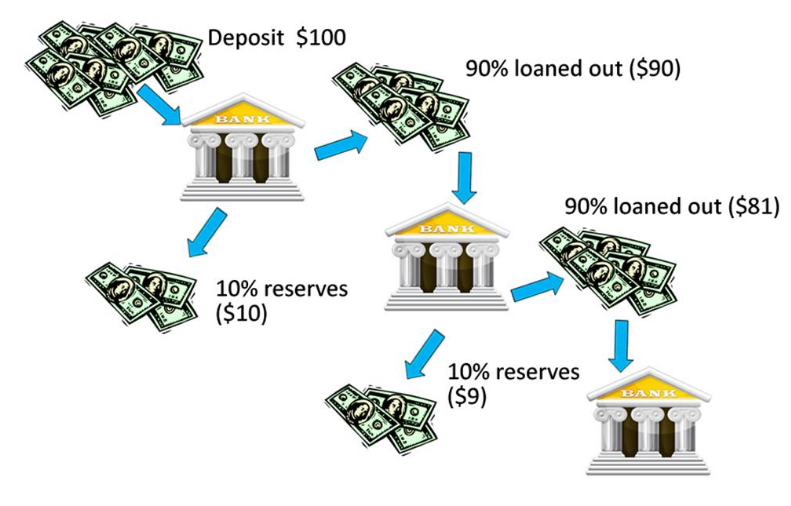
\includegraphics[width=\textwidth,height=0.2\textheight]{multiplier.png}

\begin{itemize}
\tightlist
\item
  Central Bank has the monopoly to create Central Bank Money

  \begin{itemize}
  \tightlist
  \item
    Coins, banknotes, digital euros\ldots{}
  \item
    To inject it, it exchanges it for less liquid assets
  \end{itemize}
\item
  But Monetary Base (M1) includes loans made by banks and credited to
  customers deposits.

  \begin{itemize}
  \tightlist
  \item
    Private banks create Money!
  \end{itemize}
\item
  Credit from private banks is limited by the reserve requirement ratio

  \begin{itemize}
  \tightlist
  \item
    Changing reserve ratio is a potential policy tool
  \end{itemize}
\end{itemize}
\end{frame}

\subsection{Controlling M1}\label{controlling-m1-1}

\begin{frame}{Controlling M1}
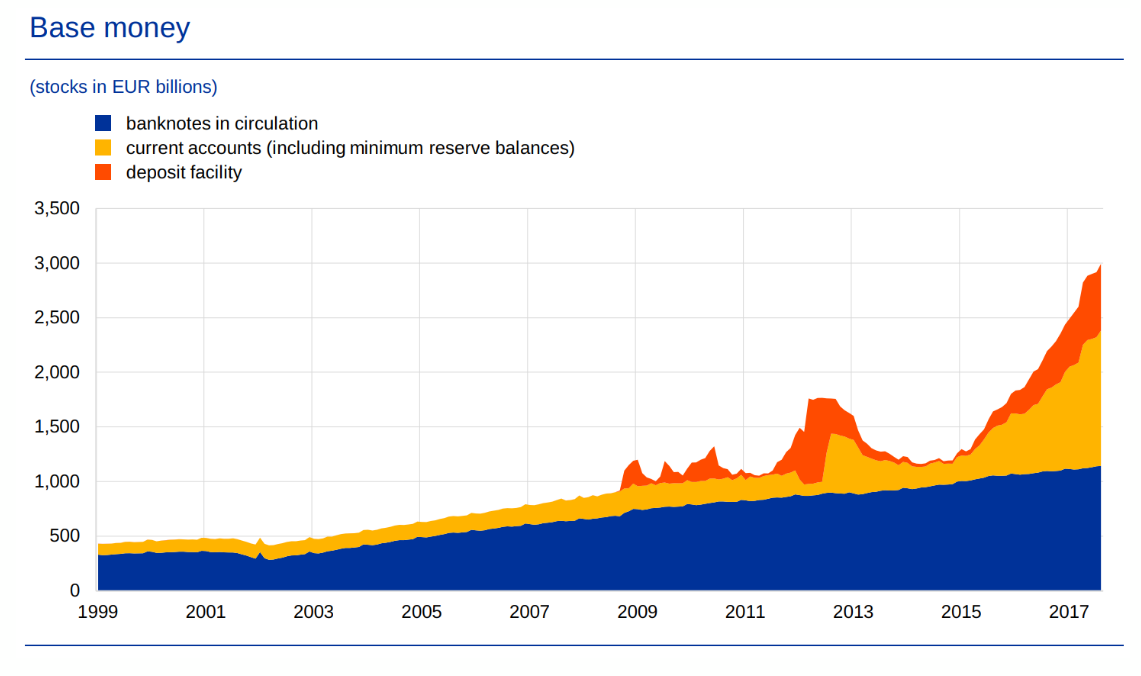
\includegraphics{base_money.png}
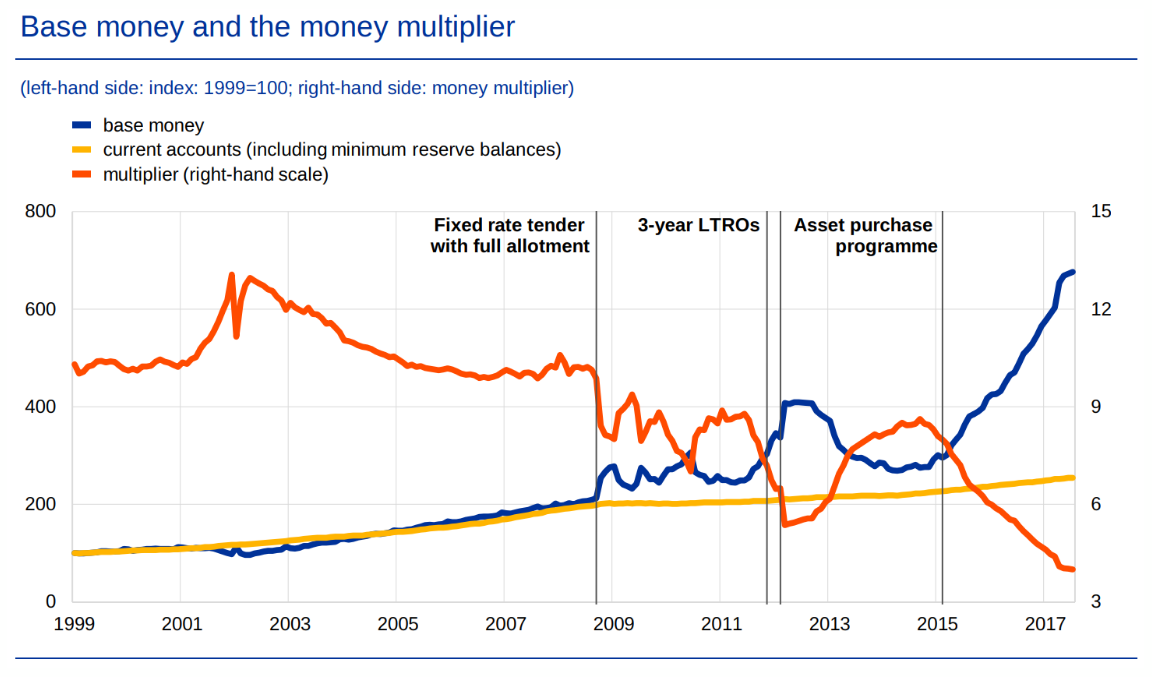
\includegraphics{base_money_multiplier.png}

Base money increased, credit not so much.\footnote{Source: ECB} Credit
multiplier has decreased and reserve requirements are not binding
(reserve requirements were 2\% until 2012, 1\% since then) The CB does
not control broad money since the financial crisis.
\end{frame}

\subsection{Evolution of Standard Policy
Practices}\label{evolution-of-standard-policy-practices}

\begin{frame}{Evolution of Standard Policy Practices}
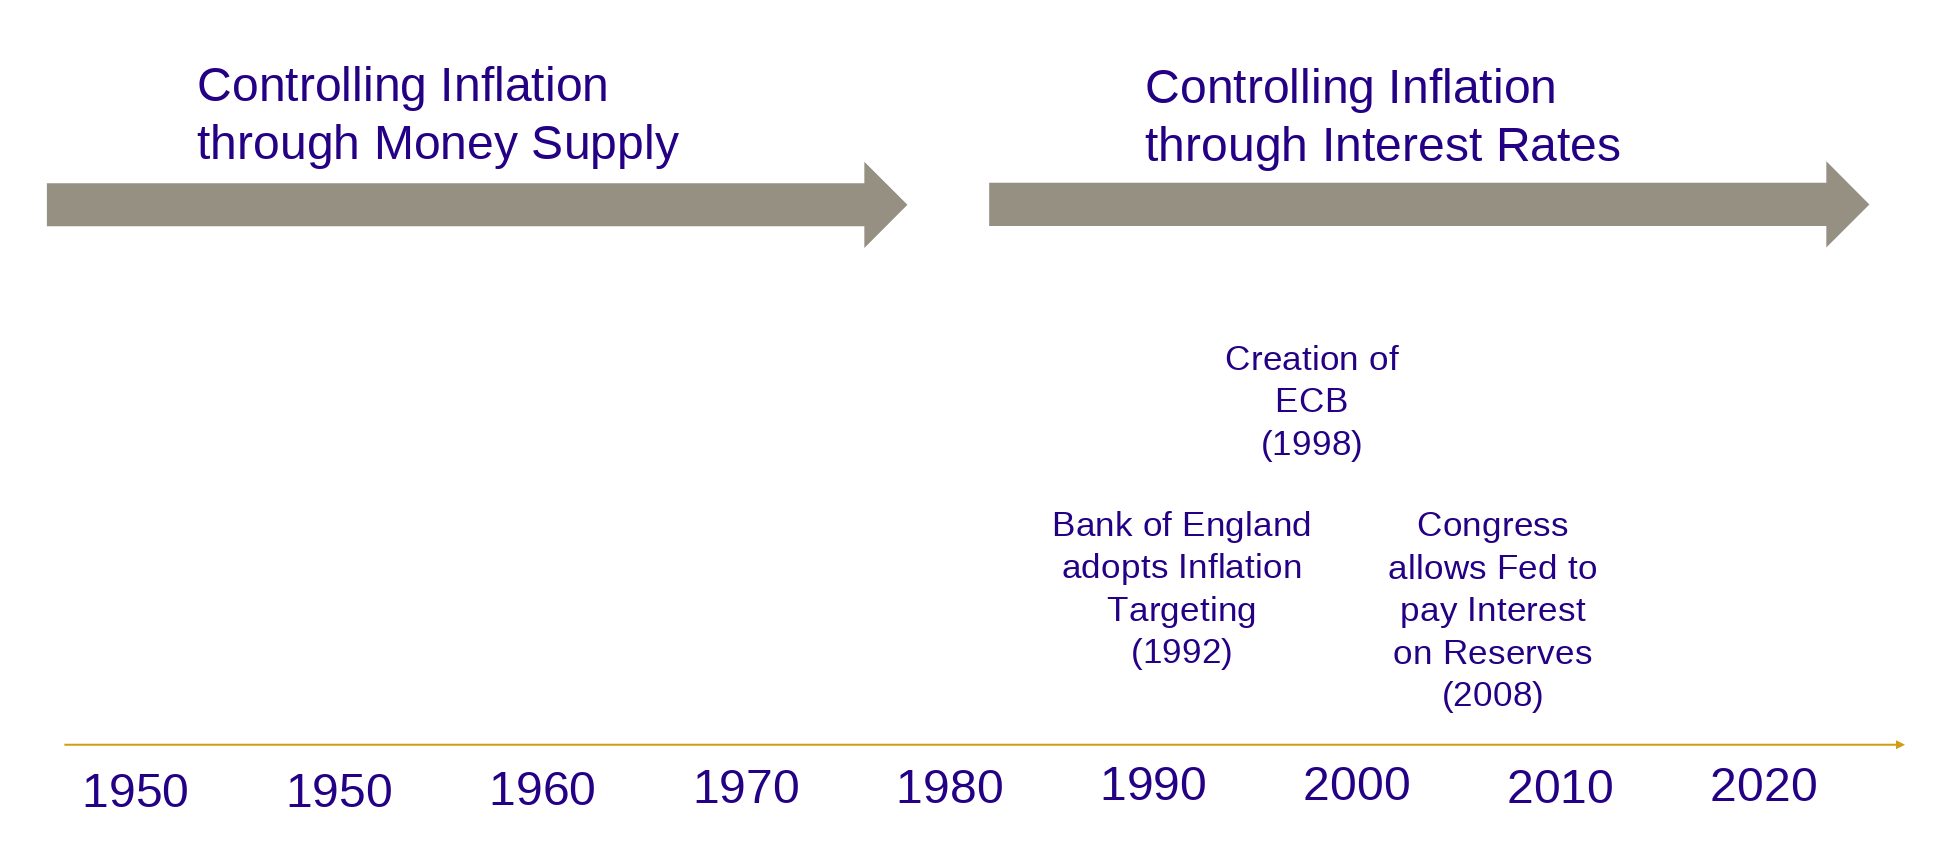
\includegraphics{evolution_practices.png}
\end{frame}

\subsection{Inflation Targeting and the Taylor
Rule}\label{inflation-targeting-and-the-taylor-rule}

\begin{frame}{Inflation Targeting and the Taylor Rule}
Most CBs have now switched to some form of ``inflation targeting'' - the
central bank tries to achieve a given inflation target (e.g.~2\% in EZ)

They achieve the target, by manipulating nominal interest rates: -
either by controlling the money supply - or by setting interest rates
directly

John Taylor, discovered empirically that interest rates decisions were
well approximated (even before inflation targeting) by a ``simple rule''
of the form:

\[i_t = i^{\star} + 0.5 (\pi_t - \pi^ {\star}) + 0.5 (y_t - y_t^ {nt})\]
\end{frame}

\subsection{Taylor Rule vs Effective
Rate}\label{taylor-rule-vs-effective-rate}

\begin{frame}{Taylor Rule vs Effective Rate}
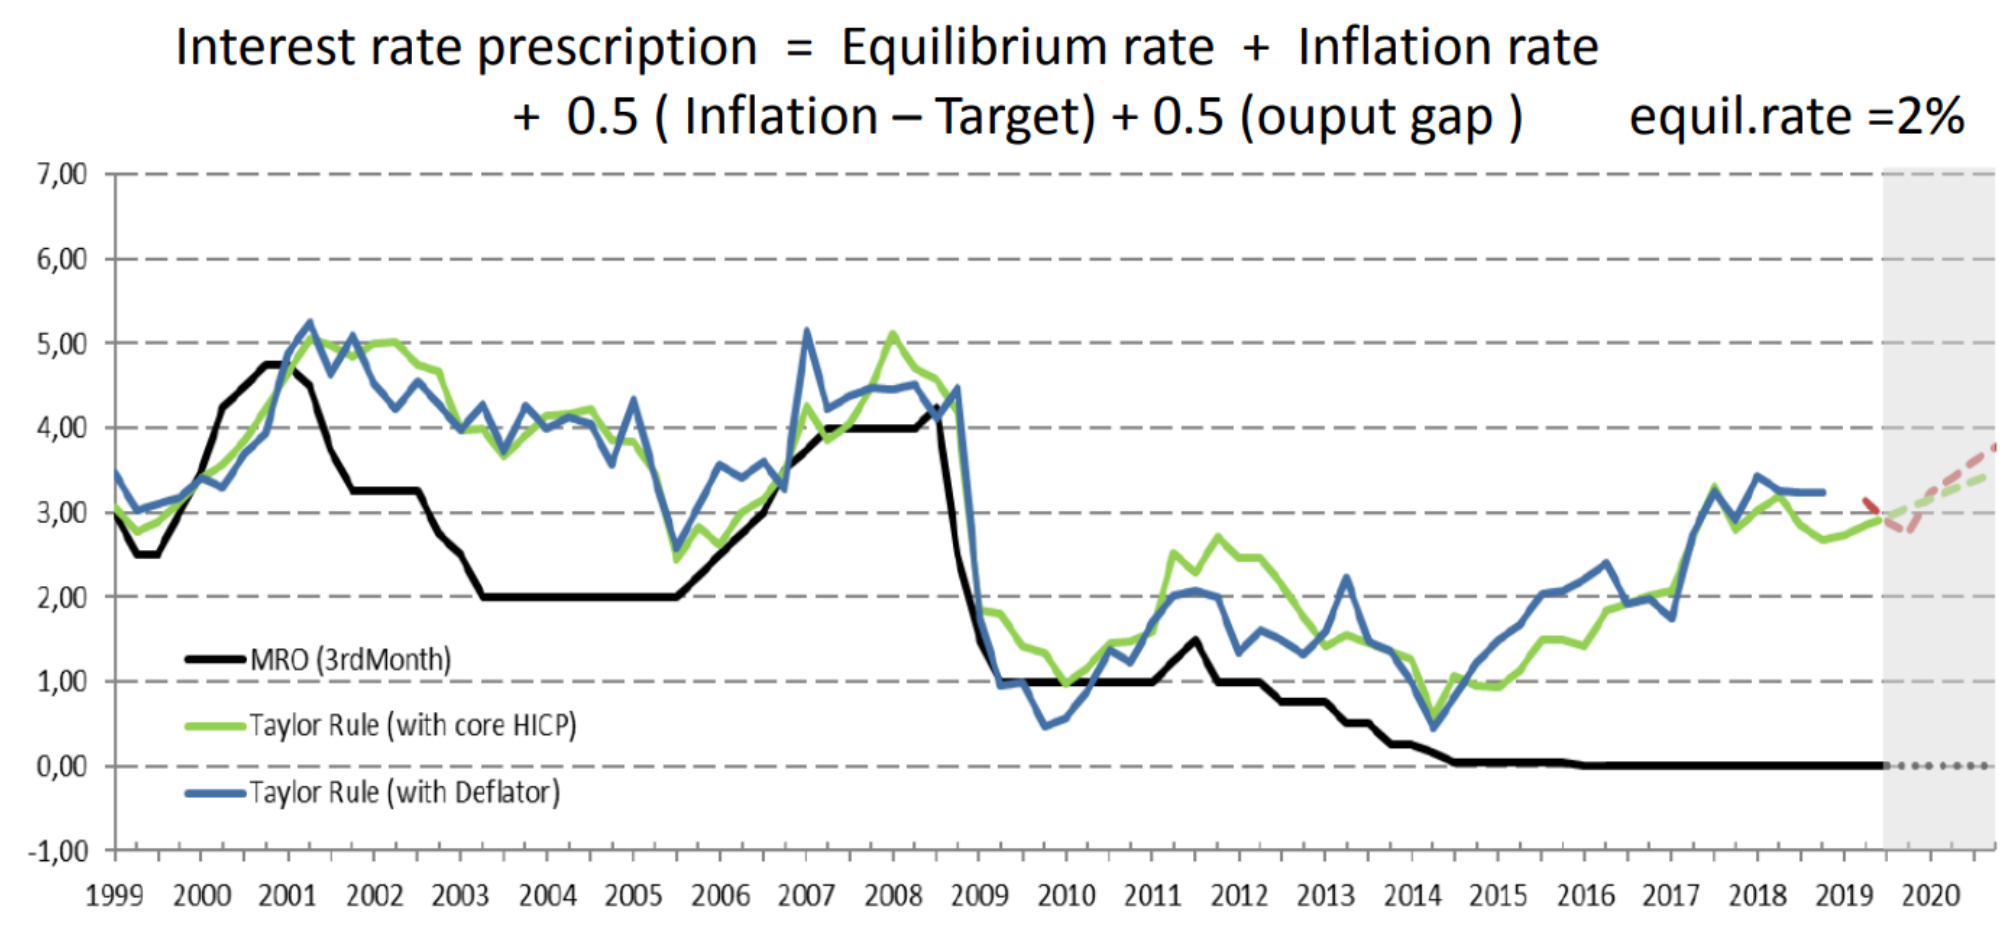
\includegraphics{taylor_rule_vs_effective_1.png}
\end{frame}

\subsection{Taylor Rule vs Effective
Rate}\label{taylor-rule-vs-effective-rate-1}

\begin{frame}{Taylor Rule vs Effective Rate}
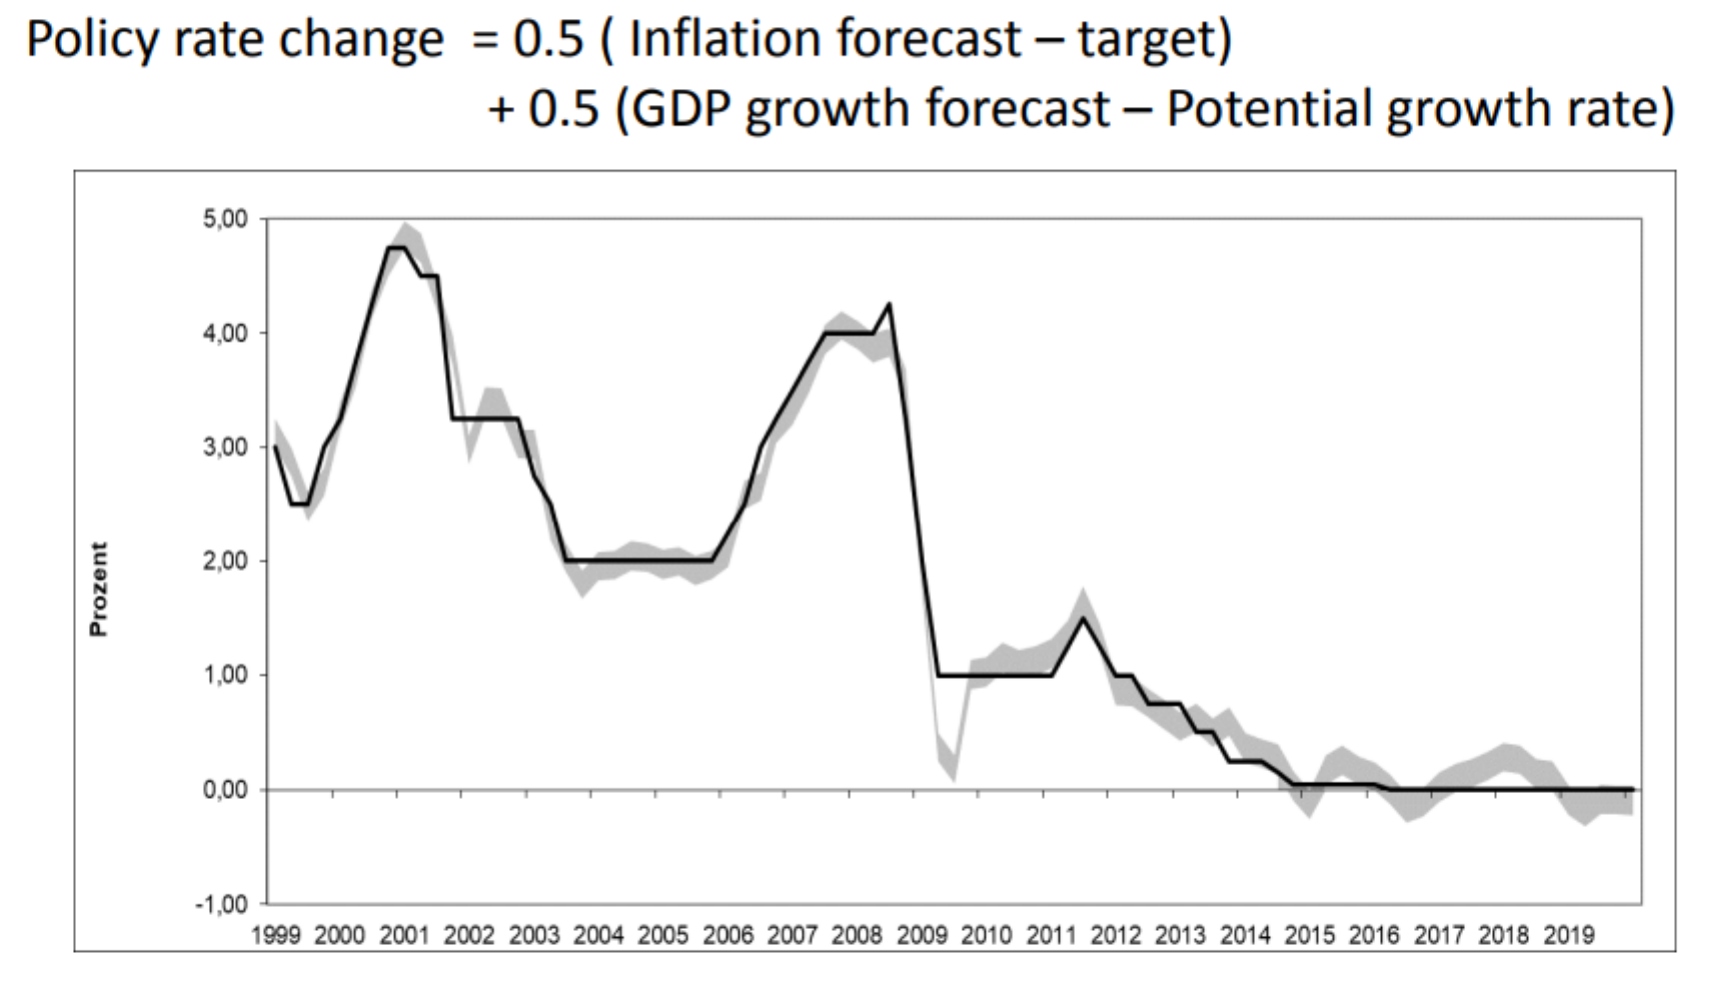
\includegraphics{taylor_rule_vs_effective_2.png}

Source: Orphanides and Wieland
\end{frame}

\subsection{The Taylor Rule}\label{the-taylor-rule}

\begin{frame}{The Taylor Rule}
Original Taylor Rule is too simple

A version based on inflation expectations describes well CB decisions:

\[i_t = i^{\star} + \alpha_{\pi} (E_t \left[ \pi_{t+1} \right] - \pi^{\star}) + \alpha_y (y_t - y_t^ {nt})\]

This version is a good reference point to understand central bank's
communication: - it uses the ``output gap'' wording to describe economic
outlook - it tries to ``anchor inflation expectations'' by keeping them
close to inflation target
\end{frame}

\subsection{Monetary Policy
Implementation}\label{monetary-policy-implementation}

\subsection{Fisher Equation and Inflation
Expectation}\label{fisher-equation-and-inflation-expectation}

\begin{frame}{Fisher Equation and Inflation Expectation}
\framesubtitle{Reminder}

Recall the Fisher equation:

\[r_t = i_t - \pi_{t+1}\]

To be more precise, we should write: \[r_t = i_t - E_t [\pi_{t+1}]\]

Because it is only the ``expected'' inflation that is known at date
\(t\). We omit the expectation sign, but keep in mind that \(\pi_{t+1}\)
represents expected inflation.
\end{frame}

\subsection{Monetary rule and inflation
expectation}\label{monetary-rule-and-inflation-expectation}

\begin{frame}{Monetary rule and inflation expectation}
We wrote real interest rule (MP) as follows:

\[r_t = r^ {\star} + \gamma (\pi_t - \overline{\pi})\]

But the CB does not directly control real interest rate. It controls the
\emph{nominal} interest rate \(i_t\).

Now, take the Fisher equation \(r_t = i_t - \pi_{t+1}\). We can replace
it above to get:
\[i_t = r^{\star} + \gamma (\pi_t - \overline{\pi}) + \pi_{t+1}\]

We see that the central bank controls a combination of inflation and
``expected inflation''. Closer to a modern Taylor Rule.

That raises interesting deep questions: how does the CB manipulate
inflation? For
later\ldots{}\footnote{Jedi Mind Trick: « These aren’t the droids you are looking for ». Matt O’Brian:  « Central Banks have a strong influence on market expectations »}
\end{frame}

\subsection{Short Term Interest Rates}\label{short-term-interest-rates}

\begin{frame}{Short Term Interest Rates}
Actually, the CB doesn't control \(i_t\) directly (the quarterly or the
yearly rate) The CB controls instead very short-term interest rates
typically overnight. Where does it happen? On the \emph{Interbank
market}:

\begin{itemize}
\tightlist
\item
  Banks lend to each others reserves they hold on a Central Bank account
\item
  Central bank is a price maker on this market How does setting a short
  term interest rate affect the long run interest rate at any maturity
  (horizon)?
\item
  Through the market's ability to \emph{arbitrage} between several
  investment options.
\end{itemize}
\end{frame}

\subsection{Arbitrage}\label{arbitrage}

\begin{frame}{Arbitrage}
\begin{columns}[T]
\begin{column}{0.48\textwidth}
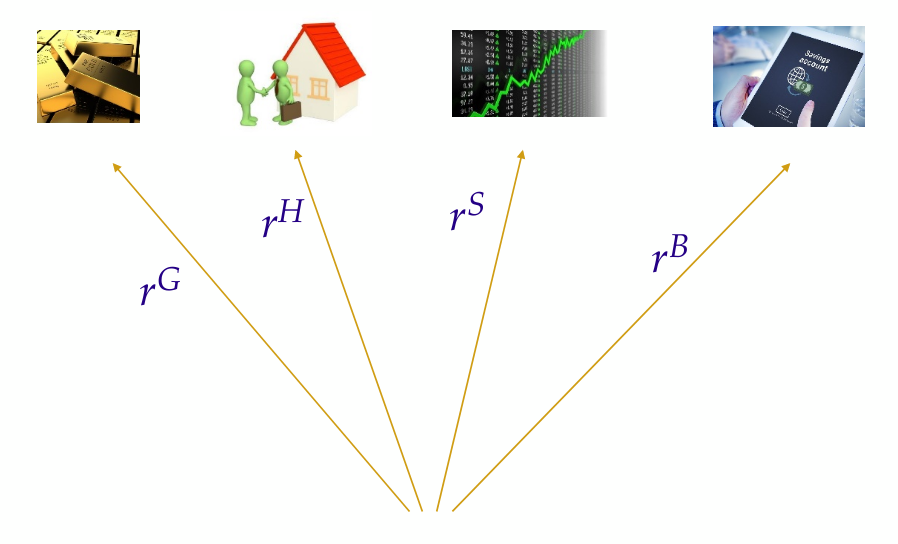
\includegraphics{arbitrage_1.png}
\end{column}

\begin{column}{0.48\textwidth}
Arbitrage is a very generic concept

When two or more equivalent investment options yield different returns
on investment, investors rush on the most profitable one\ldots{} until
returns equalize

So in equilibrium, all, equivalent investment options, must eventually
have the same return.

Diffrences between rates of return are explained by differences in:

\begin{itemize}
\tightlist
\item
  risk characteristics
\item
  liquidity
\end{itemize}
\end{column}
\end{columns}
\end{frame}

\subsection{Term Structure of Interst
Rates}\label{term-structure-of-interst-rates}

\begin{frame}{Term Structure of Interst Rates}
\begin{columns}[T]
\begin{column}{0.48\textwidth}
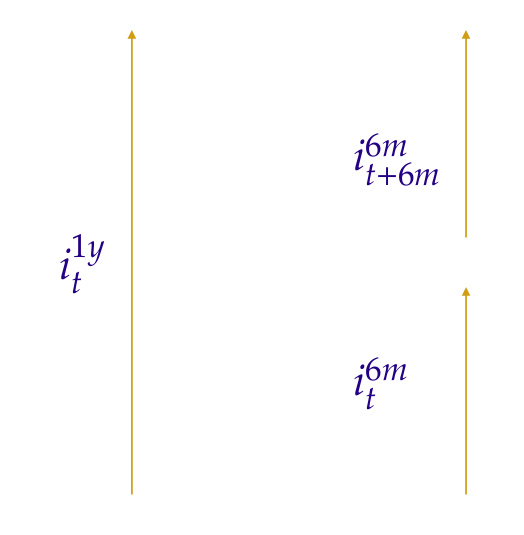
\includegraphics{arbitrage_2.png}
\end{column}

\begin{column}{0.48\textwidth}
Apply the arbitrage principle to:

\begin{itemize}
\tightlist
\item
  A one year bond yielding \(i_t^{1y}\)
\item
  Two 6 months bonds yielding (annualized)

  \begin{itemize}
  \tightlist
  \item
    \(i_t^{6m}\) bought at date \(t\)
  \item
    \(i_{t+6m}^{6m}\) bought at date \(t+6m\)
  \end{itemize}
\item
  This provides us with two options to invest over 1 year.
\item
  What is the arbitrage condition?
\end{itemize}
\end{column}
\end{columns}
\end{frame}

\subsection{Term Structure of Interest
Rates}\label{term-structure-of-interest-rates}

\begin{frame}{Term Structure of Interest Rates}
Invest value X at date \(t\)

Option 1 yields:

\begin{itemize}
\tightlist
\item
  \(X(1+i^{1y})\) after one year
\item
  (Gross) return is \((1+i^{1y})\)
\end{itemize}

Option 2 yields (pay attention to the fact that returns are annualized)

\begin{itemize}
\tightlist
\item
  \(X(1+i^{6m}_t)^{1/2}\) after 6 months
\item
  \(X(1+i^{6m}_t)^{1/2}(1+i^{t+6m}_{6m})^{1/2}\) after one year
\item
  (Gross) Return is \((1+i^{6m}_t)^{1/2}(1+i^{t+6m}_{6m})^{1/2}\)
\end{itemize}
\end{frame}

\subsection{Term Structure of Interest
Rates}\label{term-structure-of-interest-rates-1}

\begin{frame}{Term Structure of Interest Rates}
The arbitrage equation would read:
\[(1+i^{1y}) = (1+i^{6m}_t)^{1/2}(1+i^{t+6m}_{6m})^{1/2}\] Or in
log-terms:
\(i^{1y}_t = \frac{1}{2} i^ {6m}_t + \frac{1}{2} i^ {6m}_{t+6m}\) Given
that investors are risk-averse and value the flexibility of having the
cash sooner, they ask for a risk premium \(\varphi\):
\[i^{1y} = \frac{1}{2} i^{6m}{t} + \frac{1}{2} i^ {6m}{t+6m} + \varphi\]

The risk premium incorporates the uncertainty about the fact that
investment opportunities might change before one year, and about the
possibility that 6-months interest rate might change before one year.
\end{frame}

\subsection{Term Structure of Interest
Rates}\label{term-structure-of-interest-rates-2}

\begin{frame}{Term Structure of Interest Rates}
The same reasoning applies to the daily rate set by the central bank:

\[i^{1y}_t = \frac{1}{365} \left( i^{t}_{1d}  + i^{1d}_{t+1d}  + i^{1d}_{t+2d}i^{1d}_{t+2d} +  \cdots i^{1d}_{t+364d} \right) + \varphi\]

\begin{itemize}
\tightlist
\item
  By manipulating overnight interest rates (annualized term), the
  central bank can manipulate the yearly interest rate.
\item
  It does so by announcing a path for future interest rates.
\item
  For the manipulation to be effective, the path of future interest
  rates, must be clear and predictable as well as its potential
  adjustment to economic contingencies.
\item
  This is one of the reason, the central bank tries to commit to a clear
  and transparent policy.
\end{itemize}
\end{frame}

\subsection{Short Term Interest
Rates}\label{short-term-interest-rates-1}

\begin{frame}{Short Term Interest Rates}
\begin{columns}[T]
\begin{column}{0.48\textwidth}
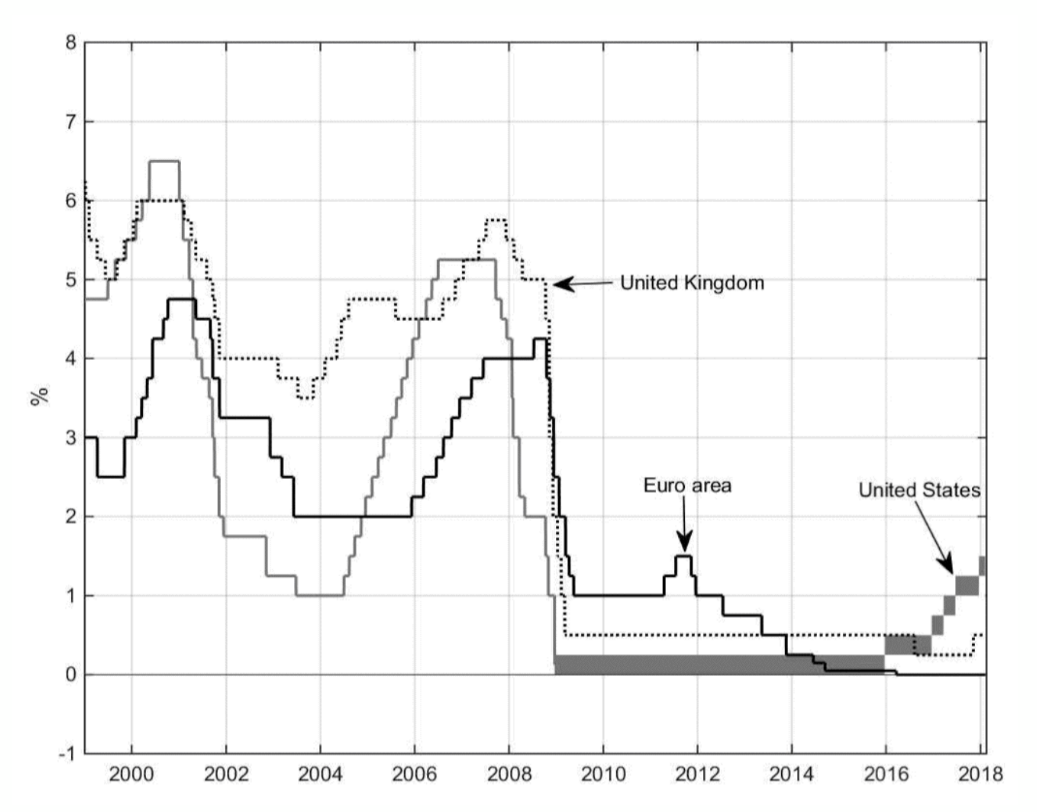
\includegraphics{short_term.png}
\end{column}

\begin{column}{0.48\textwidth}
\begin{itemize}
\tightlist
\item
  Interest rates are reviewed at a regular basis (a few months).
\item
  In general they evolve slowly, in a predictible way.
\item
  US Fed let rates fluctuate within a band.
\item
  Note that rates have stayed at historically low levels since 2008
\end{itemize}
\end{column}
\end{columns}
\end{frame}

\subsection{Short Term and Long Term Interest
Rates}\label{short-term-and-long-term-interest-rates}

\begin{frame}{Short Term and Long Term Interest Rates}
\begin{columns}[T]
\begin{column}{0.48\textwidth}
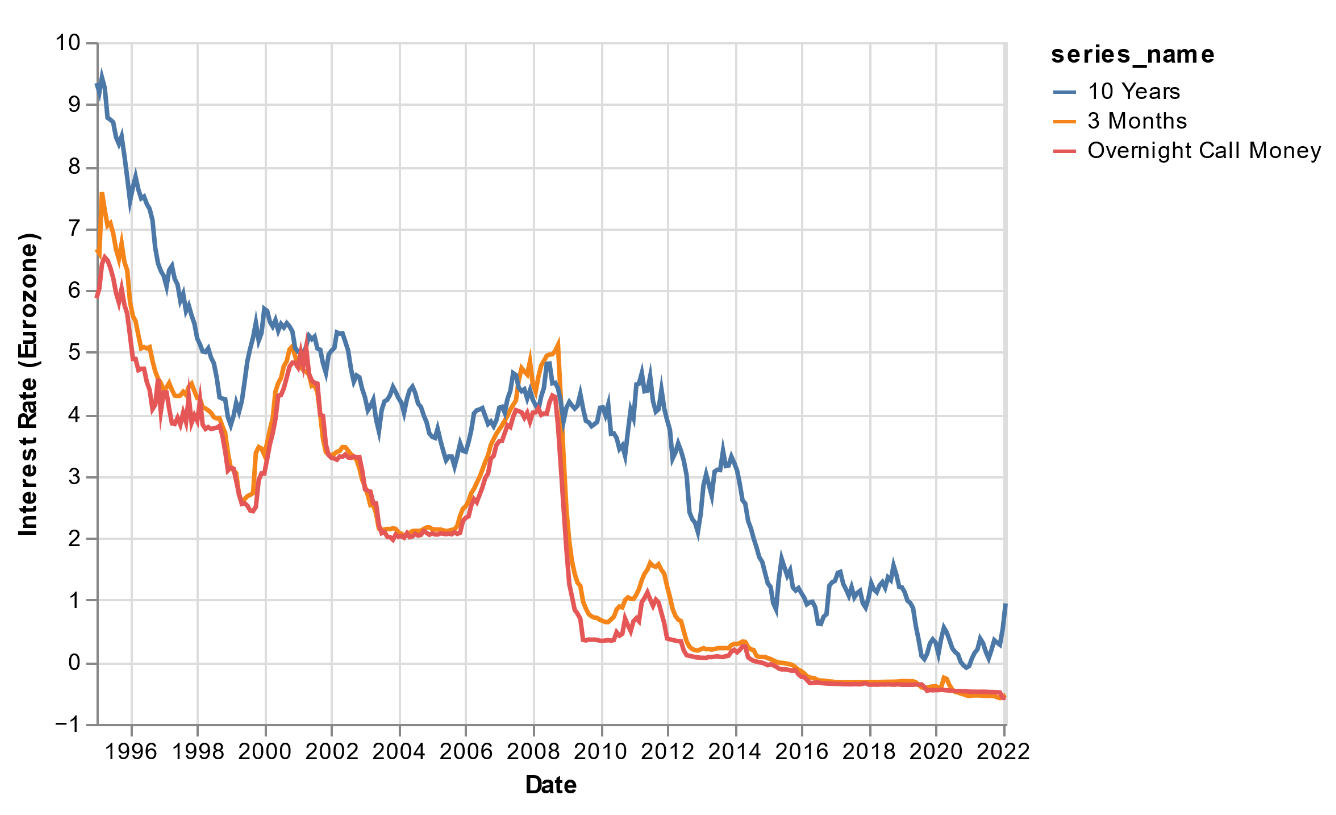
\includegraphics{short_term_long_term.png}
\end{column}

\begin{column}{0.48\textwidth}
Overnight interst rates on the interbank market, affect longer
maturities (3 months and 10 years)

Note that long term interst rates do not vary one to one with short term
interest rates.

This is because long-term interest rates incorporate \emph{future}
changes in short term interest rates.
\end{column}
\end{columns}
\end{frame}

\subsection{Interest Rate on Reserves and the Interest Rate in the
Interbank
Market}\label{interest-rate-on-reserves-and-the-interest-rate-in-the-interbank-market}

\begin{frame}{Interest Rate on Reserves and the Interest Rate in the
Interbank Market}
\begin{itemize}
\item
  So, the CB, manipulates \(r\) by manipulating \(i\) by setting the
  i.r. on the interbank market\ldots{}
\item
  But how does the CB set the price on the interbank market ? 🤔

  \begin{itemize}
  \tightlist
  \item
    It is an equilibrium price, not directly decided by the CB.
  \end{itemize}
\item
  But first, what is the role of the interbank market?

  \begin{itemize}
  \tightlist
  \item
    When clients of a given bank trade with each other no money is
    leaving the bank
  \item
    When a client of bank A pays a client of bank B, bank A should
    receive reserves from bank B
  \item
    But in the same day there might be transactions from B to A to
    offset the first transaction.
  \item
    At the end of the day imbalances to be corrected and banks need to
    pay each other
  \item
    How?
  \end{itemize}
\end{itemize}
\end{frame}

\subsection{Interest Rate on Reserves and the Interest Rate in the
Interbank
Market}\label{interest-rate-on-reserves-and-the-interest-rate-in-the-interbank-market-1}

\begin{frame}{Interest Rate on Reserves and the Interest Rate in the
Interbank Market}
\begin{itemize}
\item
  To ensure they can make the transactions to settle imbalances:

  \begin{itemize}
  \tightlist
  \item
    Banks hold reserves at the CB to cover interbank payment when needed
  \item
    And lend to each other on the interbank market
  \end{itemize}
\item
  There are two corresponding rates:

  \begin{itemize}
  \tightlist
  \item
    Reserves at the CB yield interest rate \(i^R\). Set exogenously by
    the CB.
  \item
    The market rate \(i_M\)
  \end{itemize}
\end{itemize}
\end{frame}

\subsection{Equilibrium in the Interbank
Market}\label{equilibrium-in-the-interbank-market}

\begin{frame}{Equilibrium in the Interbank Market}
What determines the amount of reserves needed by banks?

\begin{itemize}
\tightlist
\item
  Whether it is more profitable to lend to other banks or to leave
  reserves at the CB
\item
  How many transactions there are. This rises, with economic activity,
  that is \(y\)
\end{itemize}

\emph{Demand} for reserve money:
\[R^d \left( \underbrace{i^M-i^R}_{-} , \underbrace{y}_{+}\right)\]
\end{frame}

\subsection{Equilibrium in the Interbank
Market}\label{equilibrium-in-the-interbank-market-1}

\begin{frame}{Equilibrium in the Interbank Market}
\framesubtitle{Supply and Equilibrium}

The Central Bank provides liquidities to banks through open market
operations:

\begin{itemize}
\tightlist
\item
  banks exchange less liquid assets (bonds) in exchange for liquid
  central bank money (reserves)
\end{itemize}

\textbf{Supply} for reserve money is \emph{perfectly controlled} by the
CB: \[R^s\]
\end{frame}

\subsection{Equilibrium in the Interbank
Market}\label{equilibrium-in-the-interbank-market-2}

\begin{frame}{Equilibrium in the Interbank Market}
Recall the equilibrium:

\[R^S = R^D \left(i^N - i^R, y \right)\]

Inverting this relation yields:

\[i^M = i^M\left(\underbrace{i^R}_{+}, y \underbrace{R_0}_{-} \right) \geq i_R\]

The central bank has \emph{two} options to influence the interbank
interest rate:

\begin{itemize}
\tightlist
\item
  set the interest rate on reserves
\item
  introduce more CB money through open market policies
\end{itemize}

\footnote{Note: We always have $i^M>i^R$ otherwise there would be no interbank market since lending to the Central Bank would dominate completely lending to other banks (it is absolutely riskfree).}
\end{frame}

\subsection{Equlibrium in the Interbank
Market}\label{equlibrium-in-the-interbank-market}

\begin{frame}{Equlibrium in the Interbank Market}
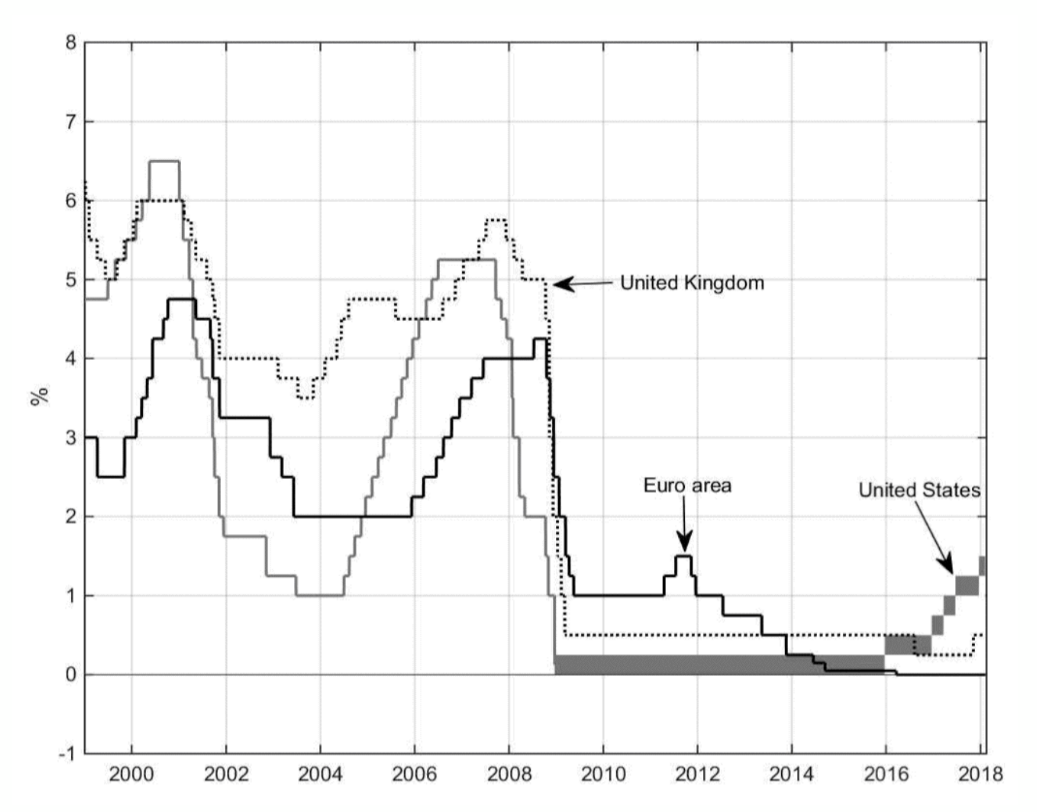
\includegraphics{short_term.png} 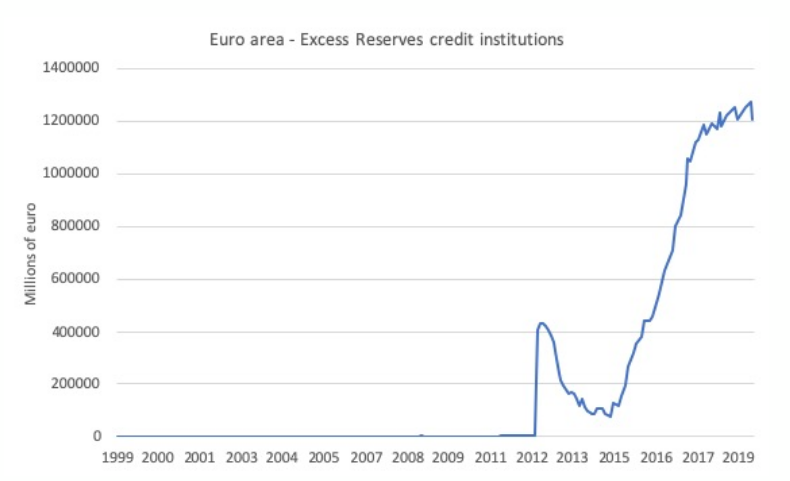
\includegraphics{excess_reserves.png}

The interest rate on reserves has become the main policy instrument.
This is a consequence of the large excess (precautionary) reserves held
by banks.

This is also true in the US where the CB remunerates excess reserves
since 2008.

\footnote{Remark: the fact that $i^M\approx i^R$ when $R^0$ is very large is implied by the demand function for reserves from previous slide.}
\end{frame}

\subsection{Takeaways}\label{takeaways}

\begin{frame}{Takeaways}
\begin{itemize}
\tightlist
\item
  Central Banks control interest rates through several policy tools
\item
  Nowadays, it concentrates on setting the interst rate on the interbank
  market
\item
  Controlling interest rate through money growth is less efficient
  because private banks don't lend enough and hold vast amounts of
  reserves at the central bank
\item
  Nowadays, interest rates on reserves held by commercial banks at the
  central bank have become the main instrument of the central bank
\item
  \ldots{} But recently, unconventional policies have brought back
  quantitative measures to the center stage.
\end{itemize}
\end{frame}



\end{document}
